\section{Grundlagen}
\subsection{Einheiten}
\vspace{-2em}
	\renewcommand{\arraystretch}{2.15}
\begin{table}[H]
	\begin{tabularx}{0.8\columnwidth}{lXX}
		Größe                     & Symbol          & Einheit                                                              \\
		\hline
		\hline
		Kapazität                 & $C$             & $F= \dfrac{\texttt{As}}{\texttt{V}}$                                 \\
		\hline
		Induktivität              & $L$             & $H = \dfrac{\texttt{Vs}}{\texttt{A}}$                                \\
		\hline
	\end{tabularx}
\end{table}
\subsection{Quadratische Formeln}
\vspace{-1em}
\begin{gather*}
x^2+px+q=0 \, \rightarrow \, x_{1/2}=-\frac{p}{2}\pm \sqrt{\left(\frac{p}{2}\right)^2-q}\\
ax^2+bx+c=0 \, \rightarrow x_{1/2} = \frac{-b\pm\sqrt{b^2-4ac}}{2a} \\
(a \pm b)^2 = a^2 \pm 2ab + b^2 \qquad 
a^2 - b^2 = (a + b)(a - b)\\
(-j\omega)^2=-\omega^2
\end{gather*}

\subsection{Logarithmische Maße/Pegel}
\textbf{Feld}größe $F_n$: Spannung, Strom\\
\textbf{Leistungs}größe $P_n$: Energie, Leistung
\begin{itemize}[leftmargin=*]
	\item \textbf{relativer Pegel}/Maß $a$ in Dezibel [dB]
	      \begin{flalign*}
		      a \,[\si{dB}]   & = 20 \cdot \lg_{} \dfrac{F_2}{F_1}  & a \,[\si{dB}]   & = 10 \cdot \lg_{}  \frac{P_2}{P_1}       & \\
		      \frac{F_2}{F_1} & =  10^{\frac{a[\si{dB}]}{20\si{dB}}} & \frac{P_2}{P_1} & =   10^{\frac{a[\si{dB}]}{10\si{dB}}}     &
	      \end{flalign*}
	\item \textbf{absoluter Pegel} $L$ mit Bezugsgrößen $ F_0, P_0 $
	      \begin{flalign*}
		      L \,[\si{dB}]   & = 20 \cdot \lg_{} \dfrac{F_1}{F_0}  & L \,[\si{dB}]   & = 10 \cdot \lg_{}  \frac{P_1}{P_0}   & \\
		      \frac{F_1}{F_0} & =  10^{\frac{L[\si{dB}]}{20\si{dB}}} & \frac{P_1}{P_0} & =   10^{\frac{L[\si{dB}]}{10\si{dB}}} &
	      \end{flalign*}
	      \renewcommand\arraystretch{1.4}
	      \begin{tabularx}{0.8\columnwidth}{l|X|X}
		      \hline
		      Einheit     & Bezugswert    & Formelzeichen        \\
		      \hline
		      dBm, dB(mW) & $ P_0 = 1mW $ & $ L_{\texttt{P/mW}}$ \\
		      dBW, dB(W)  & $ P_0 = 1W $  & $ L_{\texttt{P/W}}$  \\
		      dBV, dB(V)  & $ F_0 = 1V $  & $ L_{\texttt{V}}$ \\
		      \hline
	      \end{tabularx}
\end{itemize}

\subsubsection{Rechnen mit Logarithmen}
Rechenregeln für Logarithmen (10er-Basis): \quad $ x,y,a > 0 $
\begin{flalign*}
	\log (x\cdot y) & = \log (x) + \log (y)            & \log (\tfrac{x}{y}) & = \log (x) - \log (y)              & \\
	\log (x^{\pm a})      & = \pm a\cdot \log(x)                 & \log \sqrt[a]{x}    & = \frac{1}{a} \cdot \log (x)       & 
\end{flalign*}

\subsection{Rechnen mit Potenzen}
$a$: Basis \qquad $m,n$: Exponent
\begin{flalign*}
	& a^m \cdot a^n=a^{m+n}                                      & \frac{a^m}{a^n} & =a^{m-n} \quad(a \neq 0) & \\
	& \left(a^m\right)^n=\left(a^n\right)^m=a^{m \cdot n}        & a^n \cdot b^n   & =(a \cdot b)^n           & \\
	& \frac{a^n}{b^n}=\left(\frac{a}{b}\right)^n \quad(b \neq 0) & a^b             & = e^{b \cdot \ln a}      & \\
	& a^0 =1                                                     & a^{-n}          & = \frac{1}{a^n}          &
\end{flalign*}

\subsection{Rechnen mit Wurzeln}
$a$: Radikant \qquad $n$: Wurzelexponent\\

Merke: $\sqrt[n]{a \pm b} \neq \sqrt[n]{a} \pm \sqrt[n]{b}$ \qquad $ x = \sqrt[n]{a} = a^{\frac{1}{n}} $
\begin{flalign*}
	 & \sqrt[n]{a^m}=\left(a^m\right)^{\frac{1}{n}}=\left(a^{\frac{1}{n}}\right)^m=a^{\frac{m}{n}}=(\sqrt[n]{a})^m                                     \\
	 & \sqrt[m]{\sqrt[n]{a}}=\sqrt[m]{a^{\frac{1}{n}}}=\left(a^{\frac{1}{n}}\right)^{\frac{1}{m}}=a^{\frac{1}{m \cdot n}}=\sqrt[m \cdot n]{a}          \\
	 & \sqrt[n]{a} \cdot \sqrt[n]{b}=\left(a^{\frac{1}{n}}\right) \cdot\left(b^{\frac{1}{n}}\right)=(a b)^{\frac{1}{n}}=\sqrt[n]{a b}                  \\
	 & \frac{\sqrt[n]{a}}{\sqrt[n]{b}}=\frac{a^{\frac{1}{n}}}{b^{\frac{1}{n}}}=\left(\frac{a}{b}\right)^{\frac{1}{n}}=\sqrt[n]{\frac{a}{b}} \quad(b>0)
\end{flalign*}



\subsection{Trigonometrische Formeln}
{\small siehe Papula Mathe-FS. S.94 \& S.238 (komplexe Fkt.)}\\
\setlength{\parindent}{0pt}\\
\textbf{Komplex}:
\begin{flalign*}
	& e^{j\pi k} = (-1)^k && \pm j = e^{\pm j\frac{\pi}{2}} \quad -j=e^{j\frac{3\pi}{2}} & \\
	& e^{\pm j\omega_1 t} = \cos (\omega_1 t) \pm j \sin (\omega_1 t) && -1 = e^{\pm j\pi} \quad +1=e^{j2\pi} & \\
	& \cos  (\omega_1 t) =  \frac{e^{j\omega_1 t}+e^{-j\omega_1 t}}{2}                                    & & \sin (\omega_1 t) =  \frac{e^{j\omega_1 t}-e^{-j\omega_1 t}}{2j} &
\end{flalign*}
\textbf{Reell}:
\begin{flalign*}
	& \cos  (\omega_1 t + \frac{\pi}{2}) = - \sin(\omega_1 t)    &  & \sin  (\omega_1 t + \frac{\pi}{2}) = + \cos(\omega_1 t)           & \\
	& \cos  (\omega_1 t - \frac{\pi}{2}) = + \sin(\omega_1 t)    &  & \sin  (\omega_1 t - \frac{\pi}{2}) = - \cos(\omega_1 t)           & \\
	& \cos  (\omega_1 t \pm \pi) = -\cos(\omega_1 t)    &  & \sin  (\omega_1 t \pm \pi) = -\sin(\omega_1 t) & \\
	& \cos(\omega_1 t) = - \cos  (\pi + \omega_1 t)    &  & \sin(\omega_1 t) = \sin  (\pi - \omega_1 t)  &\\
	& \cos^2(\omega_1 t) = \frac{1}{2}[1+\cos (2 \omega_1 t)]   &  & \sin^2(\omega_1 t) = \frac{1}{2}[1-\cos (2 \omega_1 t)]   &\\
	& \frac{\sin(\omega_1t)}{\omega_1t} = \operatorname{si}(\omega_1t) = \operatorname{si}(-\omega_1t)
\end{flalign*}
\textbf{Theoreme}:
\begin{flalign*}
	& \cos^2(x) + \sin^2(x) = 1 &\\
	& \cos  (a \pm b) = \cos(a) \cdot \cos(b) \mp \sin(a) \cdot \sin(b)  &\\
	& \sin  (a \pm b) = \sin(a) \cdot \cos(b) \pm \cos(a) \cdot \sin(b)  &\\
	& \cos(2a)=\cos^2(a)-\sin^2(a)=1-2\sin^2(a) = 2\cos^2(a)-1  &\\
	& \sin(2a)=2\sin(a)\cos(a)  &
\end{flalign*}
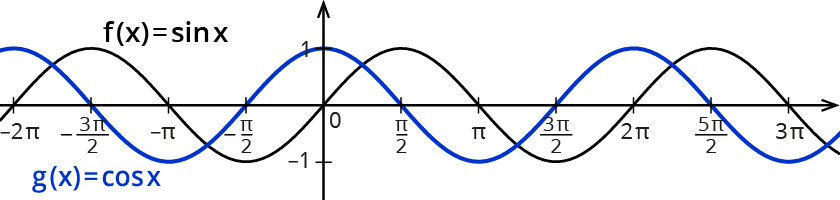
\includegraphics[width=\columnwidth]{Sinus_Kosinus_Eigenschaften}	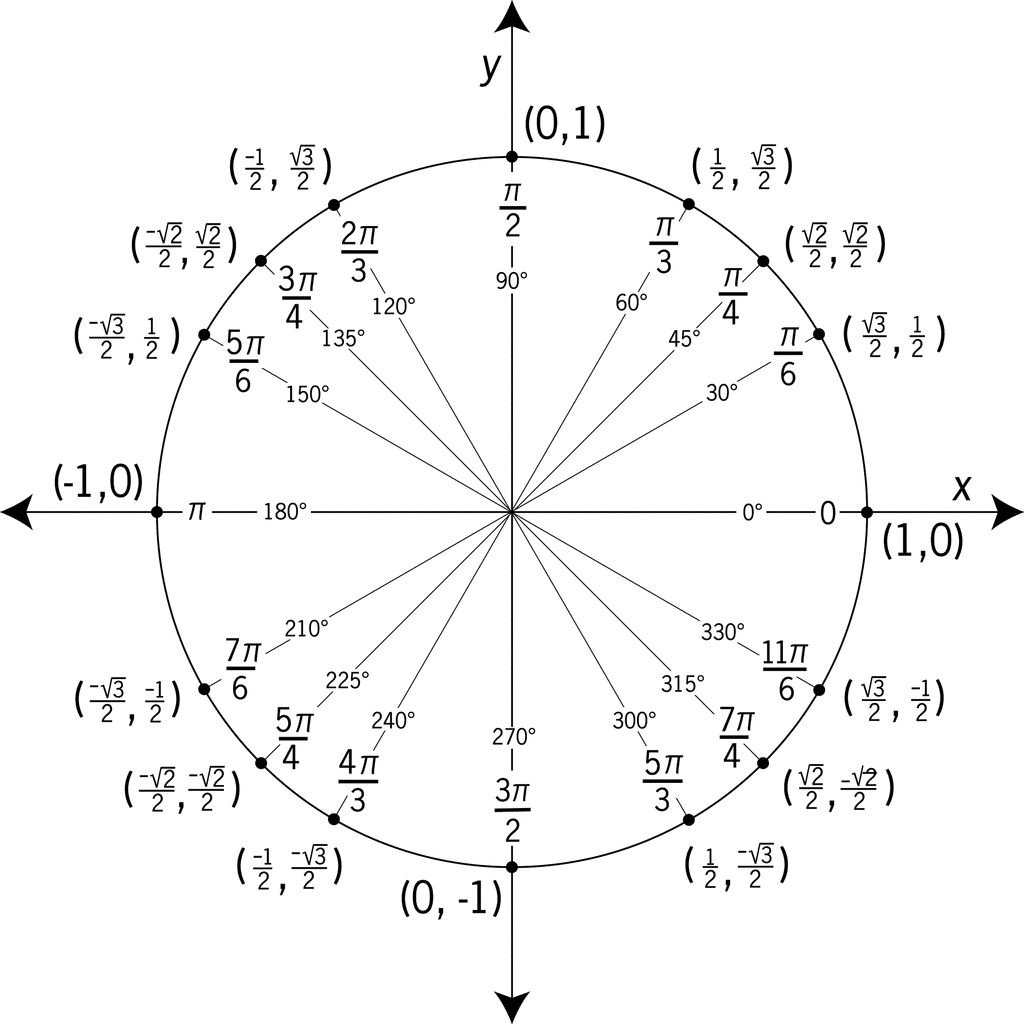
\includegraphics[width=0.65\columnwidth]{einheitskreis}